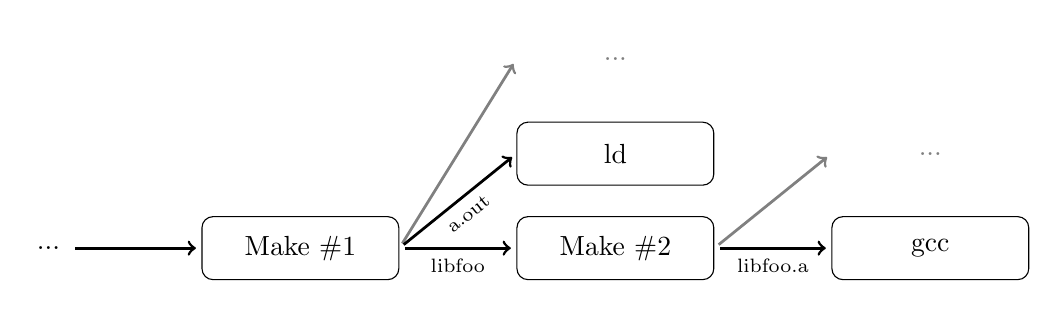
\begin{tikzpicture}
    \node (tracer) at (3.8, 0) {...};
    \node[minimum width=2.5cm, minimum height=0.8cm, style=draw, rounded corners] (make) at (7, 0) {Make~\#1};
    \node[minimum width=2.5cm, minimum height=0.8cm, gray] (child3) at (11, 2.4) {...};
    \node[minimum width=2.5cm, minimum height=0.8cm, style=draw, rounded corners] (child2) at (11, 1.2) {ld};
    \node[minimum width=2.5cm, minimum height=0.8cm, style=draw, rounded corners] (child1) at (11, 0) {Make~\#2};

    \node[minimum width=2.5cm, minimum height=0.8cm, gray] (child12) at (15, 1.2) {...};
    \node[minimum width=2.5cm, minimum height=0.8cm, style=draw, rounded corners] (child11) at (15, 0) {gcc};

    \draw[line width=1pt, shorten >=2pt, shorten <=2pt, ->] (tracer.east) -- (make.west);

    \draw[gray, line width=1pt, shorten >=2pt, shorten <=2pt, ->] (make.east) -- (child3.west);
    \draw[line width=1pt, shorten >=2pt, shorten <=2pt, ->] (make.east) -- (child2.west) node[font=\scriptsize, midway, sloped, below] {a.out};
    \draw[line width=1pt, shorten >=2pt, shorten <=2pt, ->] (make.east) -- (child1.west) node[font=\scriptsize, midway, sloped, below] {libfoo};

    \draw[gray, line width=1pt, shorten >=2pt, shorten <=2pt, ->] (child1.east) -- (child12.west);
    \draw[line width=1pt, shorten >=2pt, shorten <=2pt, ->] (child1.east) -- (child11.west) node[font=\scriptsize, midway, sloped, below] {libfoo.a};

    % \node[gray, font=\small] (text1) at (6.7, -2) {События ptrace};
    % \node[gray, font=\small] (text1) at (1, -2) {События над файлами и процессами};
    % \node[gray, font=\small] (text2) at (3.5, 1.8) {Соответствие процессов целям и граф зависимостей};
\end{tikzpicture}